\documentclass[11pt]{article}

\usepackage{graphicx}
\usepackage{grffile}
\usepackage{subcaption}

\title{Compound Interest and Simple Interest when it make an impact}
\author{Francesco Foresti}
\date{\today}

\begin{document}

\maketitle	
\tableofcontents

\newpage

\section{Introduction}

I have been contemplating the circumstances under which compound interest significantly diverges from simple interest in terms of financial returns.
\newline
To gain a clearer understanding, I plan to conduct an analysis across various scenarios, considering different expected annual returns over multiple investment horizons, specifically 10, 25, 50, 75, and 100 years. \newline
This investigation aims to delineate the thresholds at which compound interest truly manifests its impact compared to simple interest. \newline
The initial capital is always 1000\$.

\newpage

\section{Results}
Upon careful examination of the outcomes, it is evident that there is a significant disparity in returns, particularly over extended periods, which aligns with our expectations. 
\newline
However, there are two noteworthy observations:
\begin{enumerate}
    \item With a return of 2.5\%, the variance observed over a decade is minimal, amounting to    merely 2.70\%.
    \begin{figure}[ht]
    	\centering
    	\begin{subfigure}{\textwidth}
        	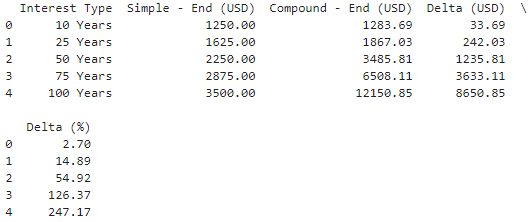
\includegraphics[width=\linewidth]{../imgs/0.025_ROI/df-0.025_ROI.png}
        	\caption{ROI: 2,5\%}
    	\end{subfigure}
	\end{figure}
    \item In the context of ultra-long-term investments, spanning over 75 years, the returns are substantially elevated. \newline
This observation prompts thoughtful consideration regarding the concept of "generational wealth." Even with a relatively modest initial investment, the potential for substantial impact on successive generations becomes apparent.
    \begin{figure}[ht]
    	\centering
    	\begin{subfigure}{\textwidth}
        	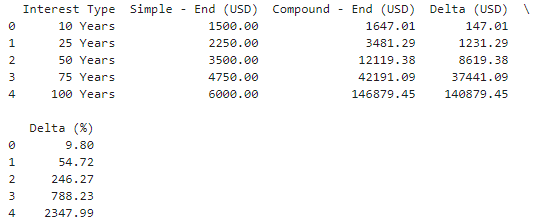
\includegraphics[width=\linewidth]{../imgs/0.05_ROI/df-0.05_ROI.png}
        	\caption{ROI: 5\%}
        	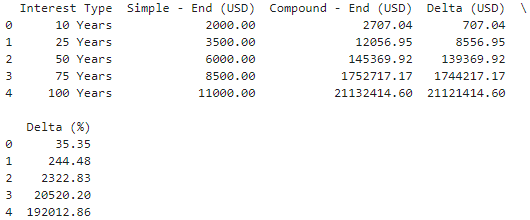
\includegraphics[width=\linewidth]{../imgs/0.1_ROI/df-0.1_ROI.png}
        	\caption{ROI: 10\%}
    	\end{subfigure}
	\end{figure}
\end{enumerate}

\end{document}